% Welcome & information slides -- OptiLänd Workshop 2026
% Compile with: latexmk -pdf welcome_slides.tex
\documentclass[aspectratio=169,11pt]{beamer}
\usetheme[progressbar=frametitle,numbering=none]{metropolis}
\setbeamersize{text margin left=0.9cm,text margin right=0.9cm}

\usepackage[utf8]{inputenc}
\usepackage[T1]{fontenc}
\usepackage{booktabs}
\usepackage{array}
\usepackage{tabularx}
\usepackage{colortbl}
\usepackage{qrcode}
\usepackage{tikz}
\usepackage{tgheros}         % clean sans font for pdflatex
\urlstyle{same}

% colours of the website
\definecolor{optiblue}{HTML}{4A6FA5}
\definecolor{optinavy}{HTML}{003056}
\definecolor{optilight}{HTML}{DCE8F7}
\definecolor{optigrey}{HTML}{F2F2F2}
\setbeamercolor{frametitle}{bg=optinavy,fg=white}
\setbeamercolor{progress bar}{fg=optiblue,bg=optilight}
\setbeamercolor{alerted text}{fg=optiblue}
\setbeamercolor{normal text}{fg=black!85}

\graphicspath{{logos/}}

\newcommand{\website}{https://jschnebel.github.io/optimization-laend.de}
\newcommand{\websiteshort}{jschnebel.github.io/optimization-laend.de}

% ---------------------------------------------------------------- layout helpers
% program table rows
\newcommand{\talk}[1]{\rowcolor{optilight}#1 & \textbf{Talks}\\}
\newcommand{\brk}[2]{\rowcolor{optigrey}{\color{black!55}#1} & \leavevmode{\itshape\color{black!55}#2}\\}
\newcommand{\evt}[2]{\rowcolor{optiblue}{\color{white}#1} & \leavevmode{\color{white}\textbf{#2}}\\}
% day heading with room
\newcommand{\dayhead}[2]{{\small\textbf{\color{optinavy}#1}}\\{\scriptsize\color{black!60}#2}\\[4pt]}
% key-value list: navy bold labels, same look on every slide
\newenvironment{infotable}[1][l]%
  {\renewcommand{\arraystretch}{1.4}\begin{tabular}{@{}>{\color{optinavy}\bfseries}l@{\hspace{10pt}}#1@{}}}%
  {\end{tabular}}
% bottom line of every content slide: small QR code + link text
\newcommand{\infolink}[2]{%
  \vfill
  {\color{optilight}\rule{\textwidth}{0.6pt}}\\[4pt]
  \begin{minipage}[c]{1.6cm}\qrcode[height=1.35cm]{\website#1}\end{minipage}%
  \begin{minipage}[c]{0.8\textwidth}\footnotesize #2\\
    {\color{optiblue}\url{\websiteshort#1}}\end{minipage}\par\vspace{2pt}}

\title{Welcome to Optimization in the Länd 2026}
\subtitle{IFIP TC7 Workshop on Optimization and Inverse Problems}
\date{25--27 November 2026 \quad\textbullet\quad Mannheim}


\begin{document}

% ---------------------------------------------------------------- title
{
\setbeamertemplate{background}{%
  % no "remember picture": works in a single pdflatex run
  \begin{tikzpicture}
    \clip (0,0) rectangle (\paperwidth,\paperheight);
    \node[anchor=center,opacity=0.18,inner sep=0pt] at (0.5\paperwidth,0.5\paperheight)
      {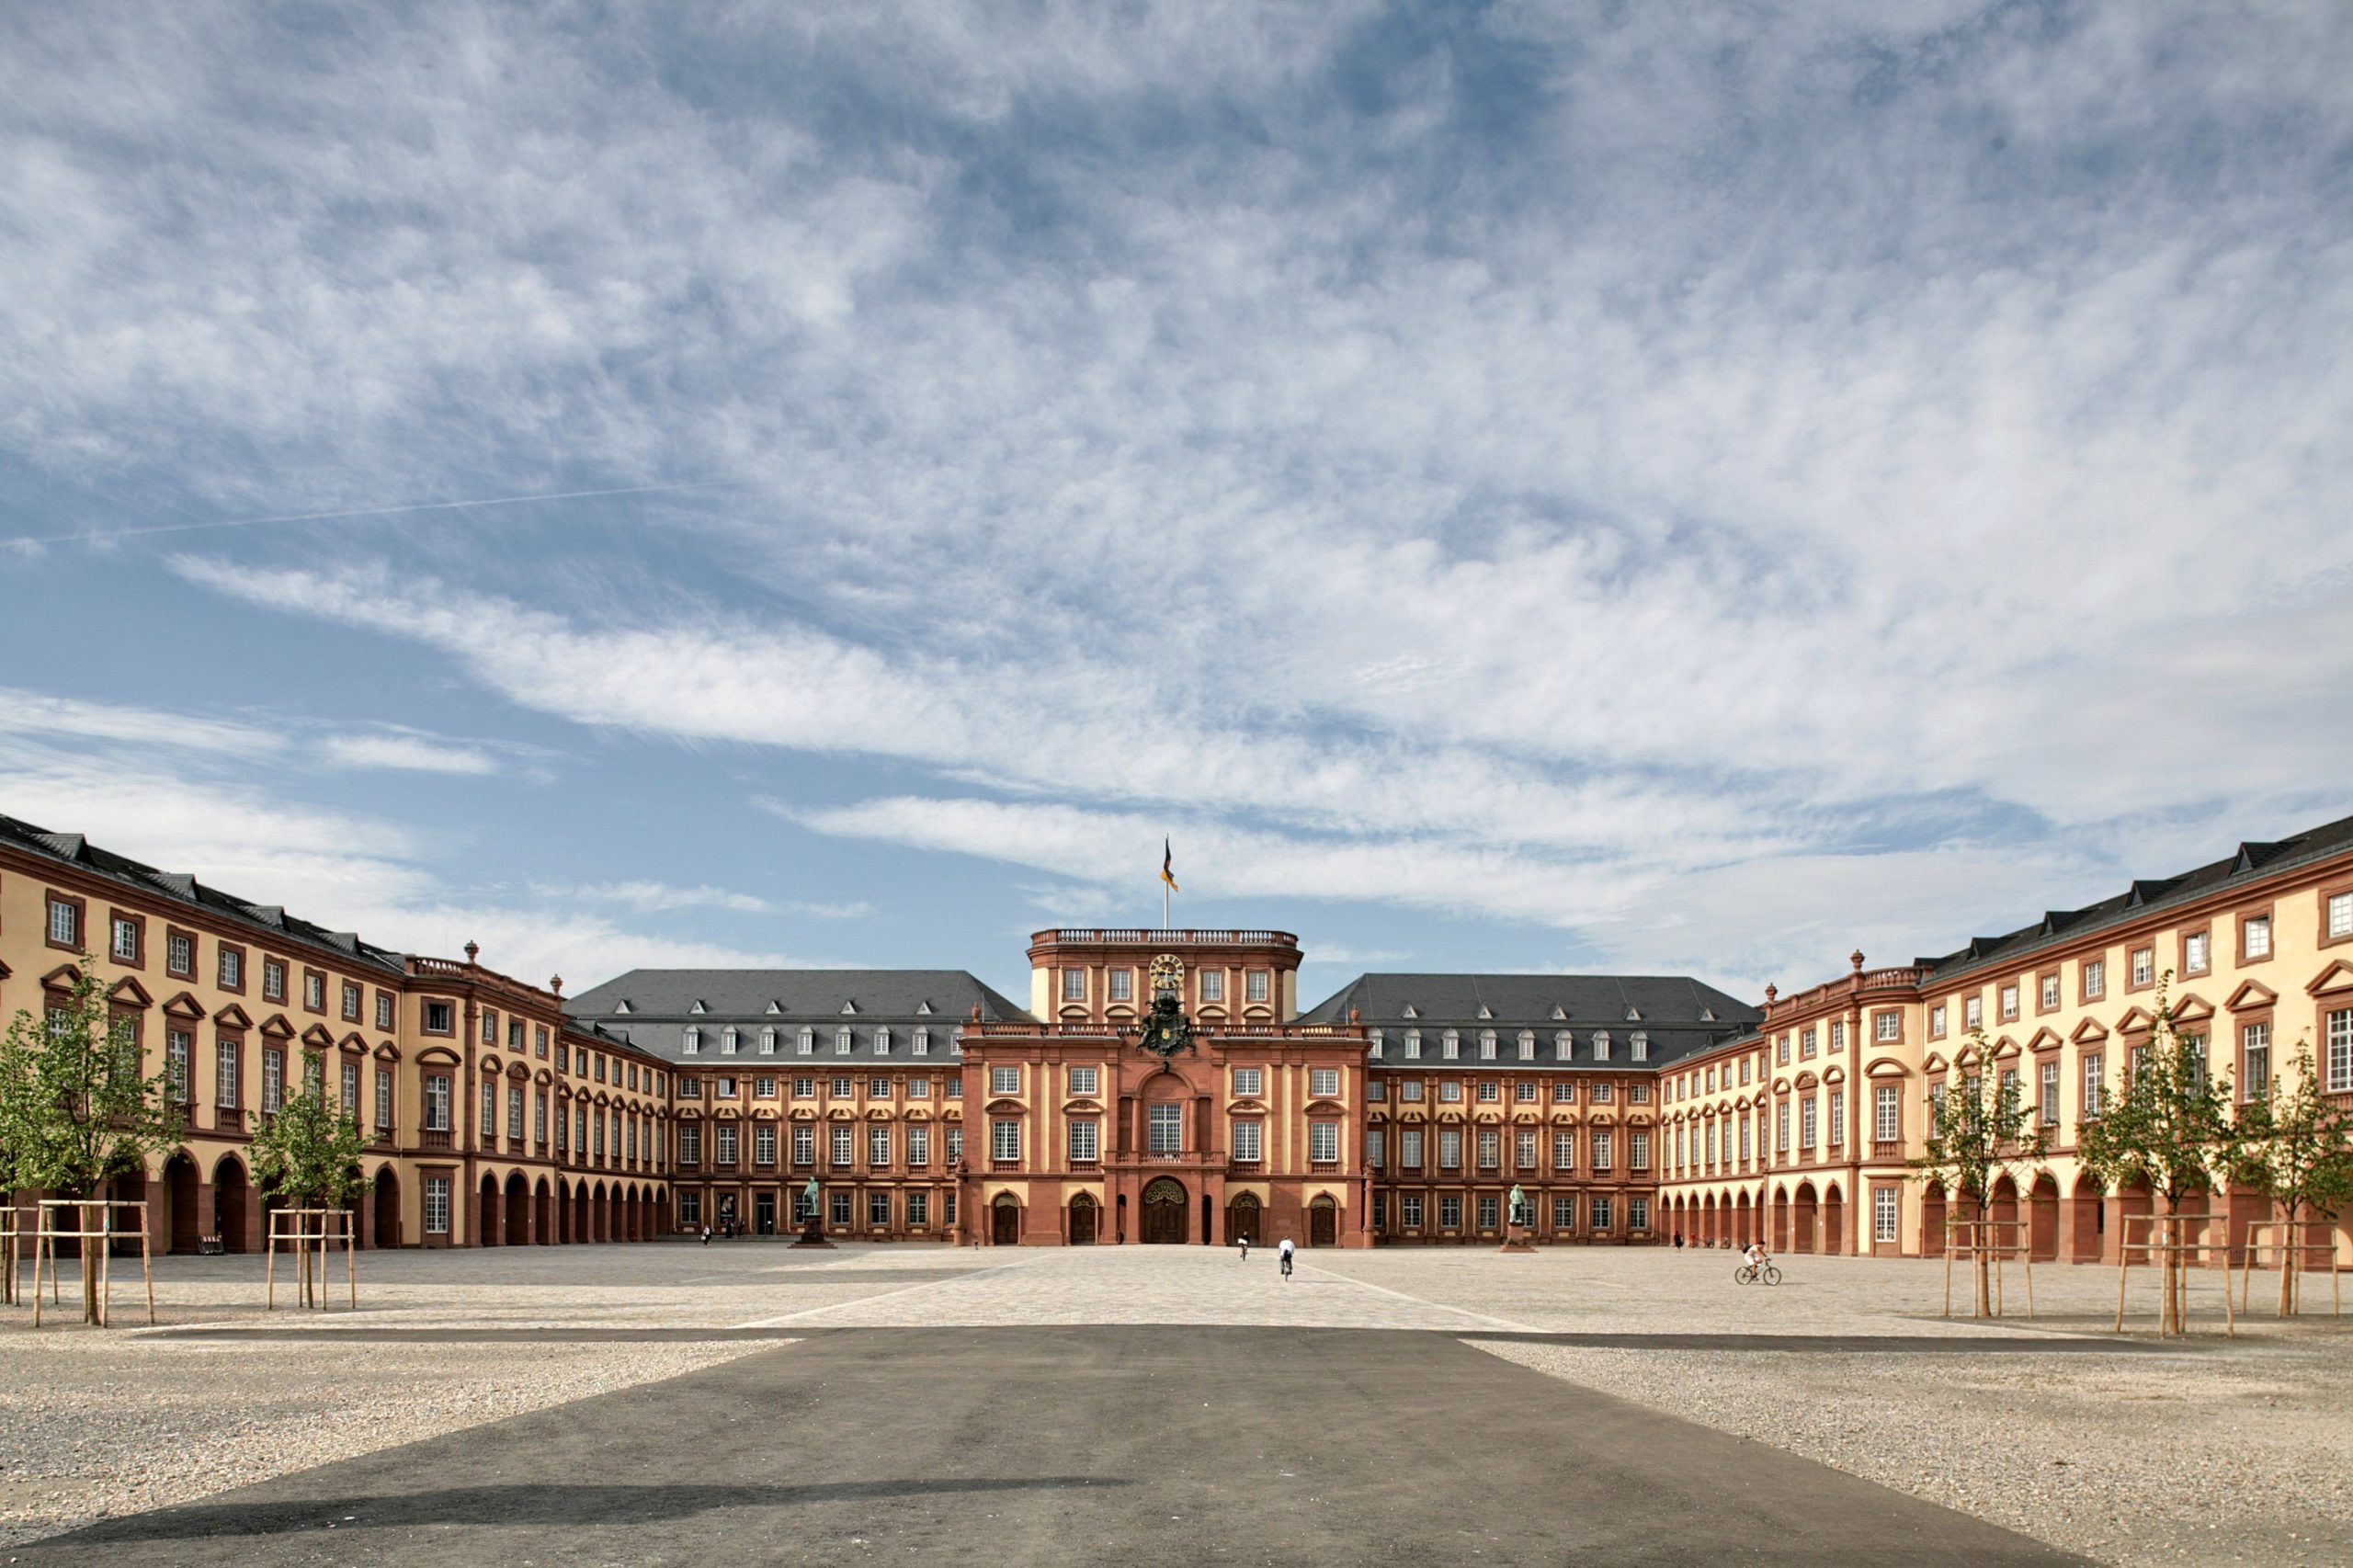
\includegraphics[width=\paperwidth]{schloss_mannheim.jpg}};
  \end{tikzpicture}}
\maketitle
}

% ---------------------------------------------------------------- program
\begin{frame}{Program at a glance}
\footnotesize
\renewcommand{\arraystretch}{1.1}
\begin{columns}[T,onlytextwidth]
\begin{column}{0.315\textwidth}
  \dayhead{Wednesday, 25 Nov}{Hörsaal B243, A5,\,6}
  \begin{tabularx}{\linewidth}{@{}l >{\raggedright\arraybackslash}X@{}}
    \brk{12:00--13:00}{Welcome}
    \talk{13:00--14:35}
    \brk{14:35--15:05}{Coffee break}
    \talk{15:05--16:40}
    \brk{16:40--17:00}{Coffee break}
    \talk{17:00--18:10}
  \end{tabularx}
\end{column}
\begin{column}{0.315\textwidth}
  \dayhead{Thursday, 26 Nov}{Fuchs-Festsaal (O\,138), Schloss}
  \begin{tabularx}{\linewidth}{@{}l >{\raggedright\arraybackslash}X@{}}
    \talk{08:35--10:10}
    \brk{10:10--10:35}{Coffee break}
    \talk{10:35--12:30}
    \brk{12:30--13:30}{Lunch break}
    \talk{13:30--15:05}
    \brk{15:05--15:30}{Coffee break}
    \talk{15:30--17:00}
    \brk{17:00--17:10}{Short break}
    \evt{17:10--18:10}{Panel}
  \end{tabularx}
\end{column}
\begin{column}{0.315\textwidth}
  \dayhead{Friday, 27 Nov}{Fuchs-Festsaal (O\,138), Schloss}
  \begin{tabularx}{\linewidth}{@{}l >{\raggedright\arraybackslash}X@{}}
    \talk{08:30--10:05}
    \brk{10:05--10:30}{Coffee break}
    \talk{10:30--11:40}
    \brk{11:40--13:10}{Lunch break}
    \talk{13:10--15:05}
    \evt{from 15:05}{Discussion \& Closing}
  \end{tabularx}
\end{column}
\end{columns}
\infolink{/program/}{Detailed program and Book of Abstracts}
\end{frame}

% ---------------------------------------------------------------- venue
\begin{frame}{Thursday \& Friday: Fuchs-Festsaal in the Palace}
\begin{columns}[c,onlytextwidth]
\begin{column}{0.4\textwidth}
  \small
  \begin{infotable}
    Room      & Fuchs-Festsaal (O\,138)\\
    Building  & Mannheim Palace\\
    Address   & Carl-Theodor-Platz\\
    Tram stop & Mannheim Schloss\\[6pt]
    Thursday  & starts at \textbf{08:35}\\
    Friday    & starts at \textbf{08:30}
  \end{infotable}
\end{column}
\begin{column}{0.57\textwidth}
  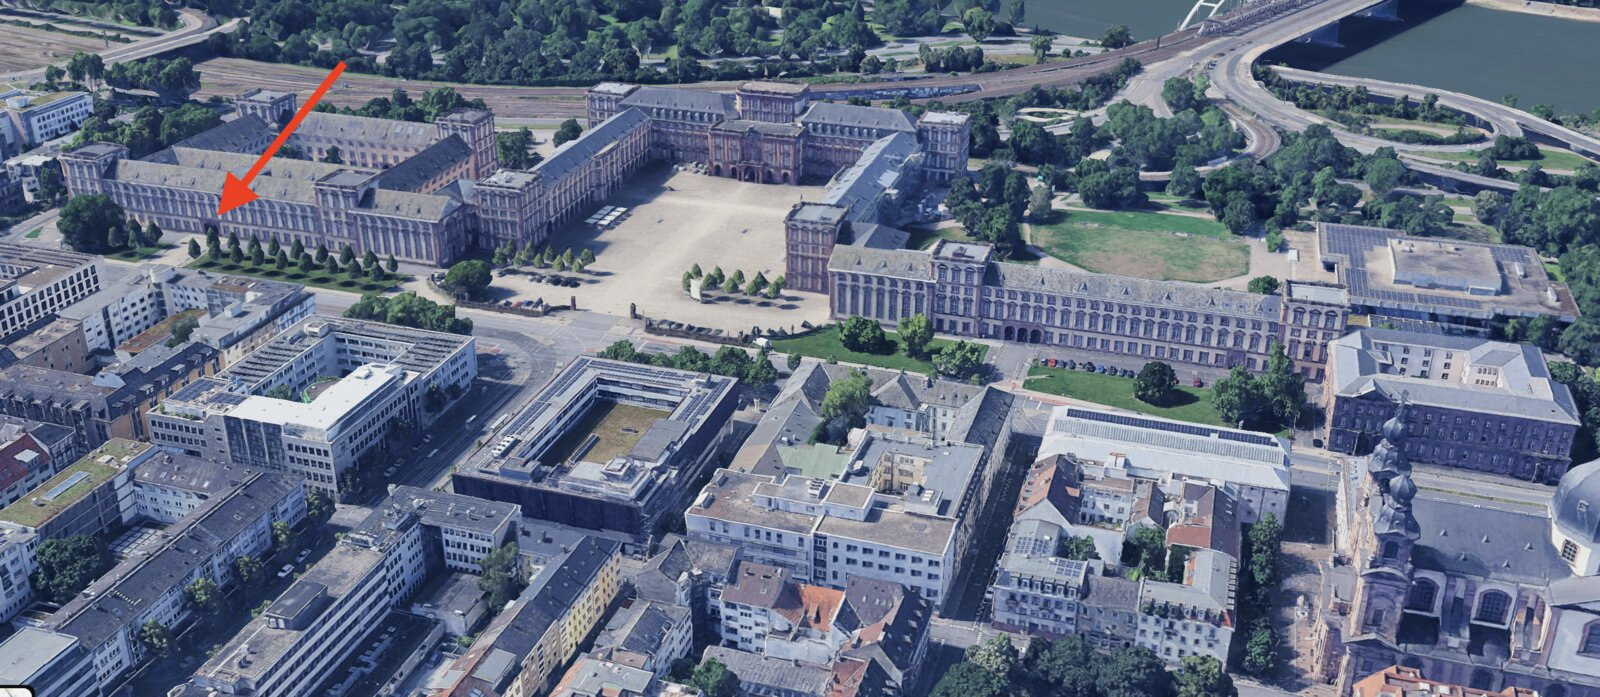
\includegraphics[width=\linewidth]{Eingang_Castle.jpg}
\end{column}
\end{columns}
\infolink{/venue/}{Maps and directions}
\end{frame}

% ---------------------------------------------------------------- food
\begin{frame}{Lunch \& dinner}
\small
Lunch and dinner are on your own -- our favourite places close to the venues are on the website.\\[10pt]
\begin{infotable}[>{\raggedright\arraybackslash}p{0.7\textwidth}]
  Lunch    & Afghan, Chinese noodles, Vietnamese, focaccia, sandwiches \& cake, burgers, \dots\\
  Dinner   & Chinese, Mexican, German, Vietnamese, \dots\\[6pt]
  Thursday & lunch break \textbf{12:30--13:30}\\
  Friday   & lunch break \textbf{11:40--13:10}
\end{infotable}
\infolink{/venue/}{All recommendations with map links (bottom of the venue page)}
\end{frame}

% ---------------------------------------------------------------- sponsors
\begin{frame}{Thank you to our sponsors}
\centering
\vfill
\begin{minipage}[c]{0.28\textwidth}\centering
  
\includegraphics[width=\linewidth]{Uni-mannheim_logo.pdf}
\end{minipage}\hfill
\begin{minipage}[c]{0.34\textwidth}\centering
  
\includegraphics[width=\linewidth]{WEB-Kopfgrafik-IWR_Desktop_EN.pdf}
\end{minipage}\hfill
\begin{minipage}[c]{0.28\textwidth}\centering
  
\includegraphics[width=\linewidth]{DFG-logo-blau.pdf}
\end{minipage}

\vspace{1.0cm}
\begin{minipage}[c]{0.16\textwidth}\centering
  
\includegraphics[width=\linewidth]{logoIFIP.png}
\end{minipage}%
\hspace{0.4cm}\begin{minipage}[c]{0.62\textwidth}
  \raggedright\small\textbf{\color{optinavy}IFIP TC\,7}: System Modeling and Optimization\\
  {\footnotesize\color{black!60}WG\,7.4 Inverse Problems \textbullet\ WG\,7.8 Nonlinear Optimization}
\end{minipage}
\vfill
\raggedright
{\color{optilight}\rule{\textwidth}{0.6pt}}\\[4pt]
\footnotesize Also supported by the \textbf{Data Science Center} of the University of Mannheim.\par\vspace{2pt}
\end{frame}
% ---------------------------------------------------------------- Announcements
\begin{frame}{GOR Working group}
\begin{itemize}
\item In 2027 the GOR will install a new working group 
\begin{verse}
Mathematical Foundations of OR
\end{verse}
\item Management team: 
\begin{enumerate}
\item Marc Goerigk (University of  Passau) 
\item Johannes Thürauf (University of Technology Nuremberg) 
\item Mathias Staudigl (Vienna University of Economics and Business)
\end{enumerate} 
\end{itemize}
\end{frame}

\begin{frame}{Workshop announcement} 
	\begin{columns}
\begin{column}{0.45\textwidth}
\begin{block}{}
\textbf{Opening Workshop announcement}
\begin{itemize}
\item Kick-Off event on November 17-19, 2027
\item Venue: Campus WU Wien 
\item You are all invited to come and present your best work. Stay tuned for updates. 
\end{itemize}
\end{block} \end{column}
\begin{column}{0.45\textwidth}
\begin{block}{}		
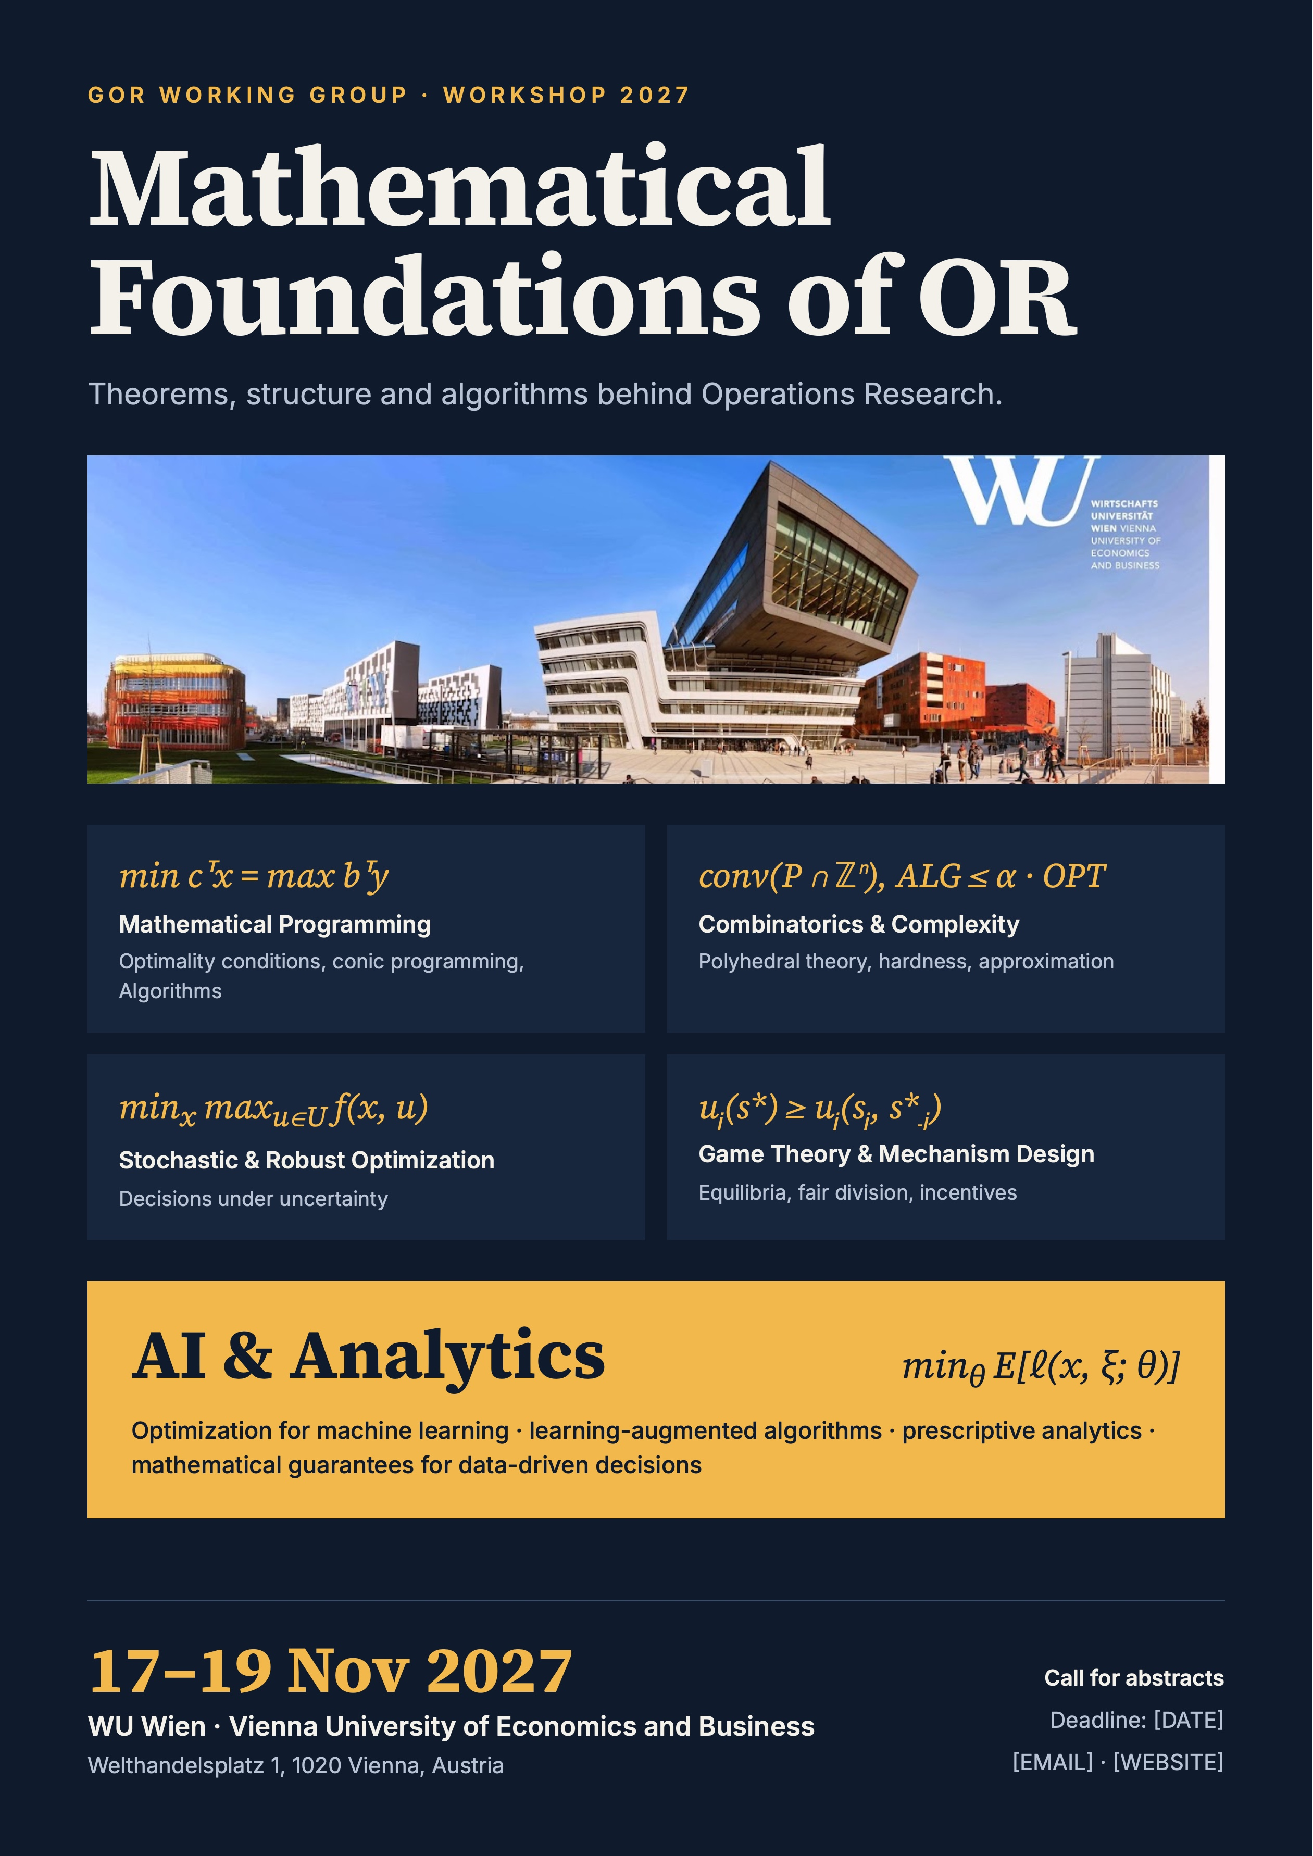
\includegraphics[scale=0.2]{GORPoster.pdf}
\end{block}\end{column}\end{columns}
\end{frame}

\begin{frame}{PhD Opportunities} 
Department of Business Analytics and Decision Sciences
\vspace{0.4cm}

Part-time, 30 hours/week
Starting January 01, 2027, and ending after 6 years

We offer 4 PhD positions on decision-making in complex, uncertain, and strategic environments. Possible topics combine methods such as optimization, game theory, AI search, heuristics, and machine learning with applications in energy, scheduling, healthcare, revenue management, transportation, and timetabling.

\vspace{0.4cm} 

Another round of hirings will start early 2027. 

\end{frame}


\end{document}
